\documentclass[/home/jesse/Analysis/FemtoAnalysis/AnalysisNotes/AnalysisNoteJBuxton.tex]{subfiles}


\begin{document}

\subsubsection{Discussion of \mt-Scaling}
\label{ResultsLamK_DiscussionOfmTScaling}

It is clear from the results presented in the previous sections, that the \LamK systems do not conform to the approximate \mt-scaling of the pair source sizes. 
At first thought, this may appear to be a troubling result; the approximate scaling is an observed consequence of the collective behavior of the soft (low-\pt) sector of the produced system.
The \Lam and K  particles certainly participate in the collective expansion of the QGP medium, so why do their extracted femtoscopic radii not behave as expected?
To get straight to the point: the \LamK systems are (obviously) comprised on non-identical particles, each with its own and unique single particle source.
Each source is, in general, unique in both its overall size, and in its space-time position within the produced medium.
The hydrodynamic nature of the medium produces the approximate \mt-scaling with respect to these single-particle sources, not the pair sources.
The combination of these effects, when probing correlations between non-identical particle pairs, leads to extracted radii falling outside of the (identical particle femtoscopy) \mt-scaling trend.
Figure \ref{fig:mTScalingOfRadii_3ReswIndmTCartoon} (which contains the same data as Fig.\ref{fig:mTScalingOfRadii_3Res}), shows again the $R_{\mathrm{inv}}$ vs \mt plot, but also highlights (with arrows) the approximate individual $\langle m_{\mathrm{T}} \rangle$ values of the single particle distributions.
The grey circles show how to single particle sizes change with \mt.

Taking a close look at Fig. \ref{fig:mTScalingOfRadii_3ReswIndmTCartoon}, one can see that the previously published data (transparent points) are for identical particle analyses only.
For these cases, the pair source, probed through femtoscopy, is comprised of two identical sources laying on top of each other.
The extracted femtoscopic radii are related to the single particle source sizes by a factor of $\sqrt{2}$, and of course follow the \mt-scaling trend.
The other (unpublished) non-identical particle femtoscopic study (p\Lam) included in the figure, also shows radii deviating from the \mt-scaling band.
Drawing a comparison with the $\Lambda\bar{\Lambda}$ study shown in Fig. \ref{fig:mTScalingOfRadii_3Res} is a bit more complicated; the $\Lambda\bar{\Lambda}$ system, although containing non-identical particles, does contain a particle with its antiparticle, for which annihilation could conceivably alter the pair source distribution.
It would be more surprising if the non-identical analyses did happen to conform to the scaling; although, this could occur for a non-identical analysis in which the particles have similar masses as well as similar \mt distributions.
For the case presented here, the result differing from \mt-scaling is not surprising. 


\begin{figure}[h]
  \centering
  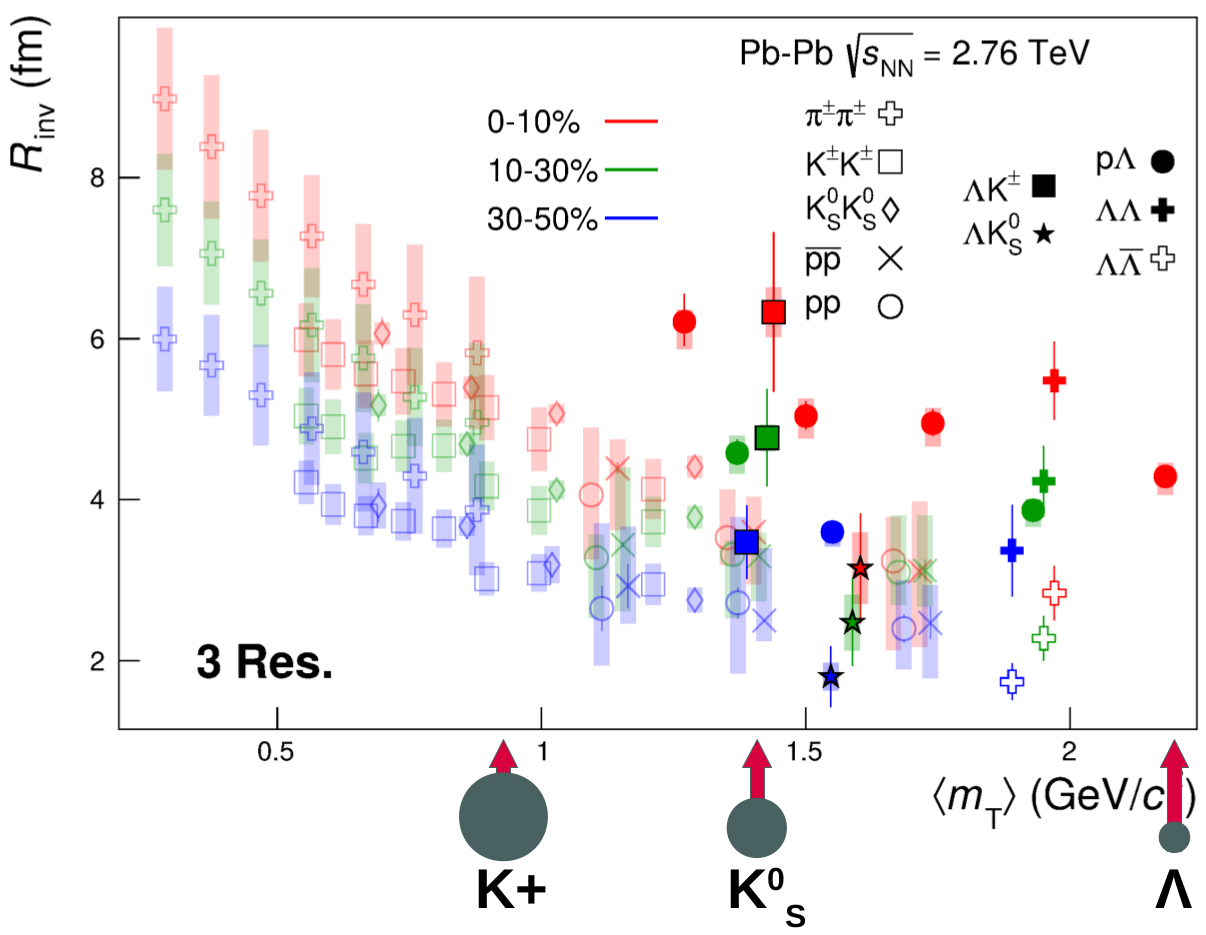
\includegraphics[width=0.75\textwidth]{/home/jesse/Analysis/FemtoAnalysis/AnalysisNotes/7_ResultsAndDiscussion/7.1_ResultsLamK/7.1.5_ResultsLamK_DiscussionOfmTScaling/OtherFigures/mTScalingwIndmTCartoon.png}
  \caption[$m_{\mathrm{T}}$ Scaling of Radii: 3 Residuals in Fit (with individual \mt highlighted)]{Same as Fig. \ref{fig:mTScalingOfRadii_3Res}, but with the individual \mt values for the single particle distributions identified.  The grey circles show how the single particle sizes are expected to change with \mt.}
  \label{fig:mTScalingOfRadii_3ReswIndmTCartoon}
\end{figure}


I will also briefly point out that it is not automatically clear where a non-identical study should be placed on such a $R_{\mathrm{inv}}$ vs \mt plot.
Each single particle distribution has a well-defined $\langle m_{\mathrm{T}} \rangle$, which, to a large extent, determines the single particle region of homogeneity.
When combining two sources with different spatio-temporal characteristics, originating from particles of different \mt, how should one define the pair \mt?
A simple mathematical expression for the pair \mt is easy to come up with, but that's not exactly what I'm hinting at here.
With respect to this \mt-scaling picture, the \mt value dictates the source size, and one desires the same for non-identical particles.
However, do the two unequal sized sources both contribute equally to the extracted femtoscopic size?
Or does the larger (smaller) source more closely dictate the femtoscopic signal?
If the contribution is equal, then it seems natural to simply more-or-less average the two, single particle, \mt values.
If the contribution is unequal, then there should be introduced some sore of weighting in the pair \mt calculation reflecting this fact.
In any case, in our study we use the most straightforward definition of pair \mt, defined as:


\begin{equation}
 m_{\mathrm{T, pair}}^{2} = \left( \frac{m_{\mathrm{inv}}}{2} \right)^{2} + \left( \frac{1}{2} |\textbf{\textit{p}}_{\mathrm{T,1}} + \textbf{\textit{p}}_{\mathrm{T,2}}| \right)^{2}
\label{eqn:PairmTv1}
\end{equation}

Many times, the equation for non-identical particle pair \mt is defined with the average mass replacing $m_{\mathrm{inv}}/2$.  However, the above Eq. \ref{eqn:PairmTv1} is more directly analogous to the single particle \mt:

\begin{equation}
 m_{\mathrm{T}}^{2} = m^{2} + \textbf{\textit{p}}_{\mathrm{T}}^{2} = (p^{0})^{2} - (p^{3})^{2}
\label{eqn:SinglemT}
\end{equation}

as, Eq. \ref{eqn:PairmTv1} may be rewritten as:



\begin{equation}
\begin{aligned}
m_{\mathrm{T, pair}}^{2} &= (K^{0})^{2} - (K^{3})^{2} \\
K^{\mu} & \equiv \frac{1}{2} \left( p_{1}^{\mu} + p_{2}^{\mu} \right)
\end{aligned}
\label{eqn:PairmTv2}
\end{equation}



Identical particle femtoscopic studies are able to probe only the size of the emitting region, or, more precisely, the second moments of the emission function.
In addition to this, non-identical particle studies are able to measure the relative emission shifts, the first moments of the emission function.
One method to extract information about the emission asymmetries in the system is via a spherical decomposition of the correlation function.
With this method, one can draw a wealth of information from just a few components of the decomposition.
More specifically, the $C_{00}$ component is similar to the 1D correlation functions typically studied, and probes the overall size of the source.
The $\Im C_{11}$ component probes the asymmetry in the system; a non-zero value reveals the asymmetry. 

In Fig. \ref{fig:LamKchP_ReC00C11_0010} we show results for the $C_{00}$ and $\Im C_{11}$ components from the spherical decomposition of our \LamKchP system in the 0-10\% centrality bin (red circles).
Results from a number of other components within the decomposition, as well as for our \LamKs and \LamKchM systems, are contained in \ref{AdditionalFigures_SphericalHarmonics}.
Along with the experimental data in Fig. \ref{fig:LamKchP_ReC00C11_0010}, we have also included results from THERMINATOR simulation for an impact parameter of b = 2 fm (gold stars).
As THERMINATOR does not include any final state effects, we assumed scattering parameters ($\Re f_{0}, \Im f_{0}, d_{0}$) = (-1.16, 0.51, 1.08) and weighted the numerator pairs with $|\Psi|^{2}$, as discussed previously.
As seen in the figure, the $C_{00}$ signal is similar to that observed in our one-dimensional study.
The $\Im C_{11}$ component shows a clear deviation from zero, and the negative value signifies that the \Lam particles are, on average, emitted further out and/or earlier than the K mesons.



\begin{figure}[h!]
  \centering
  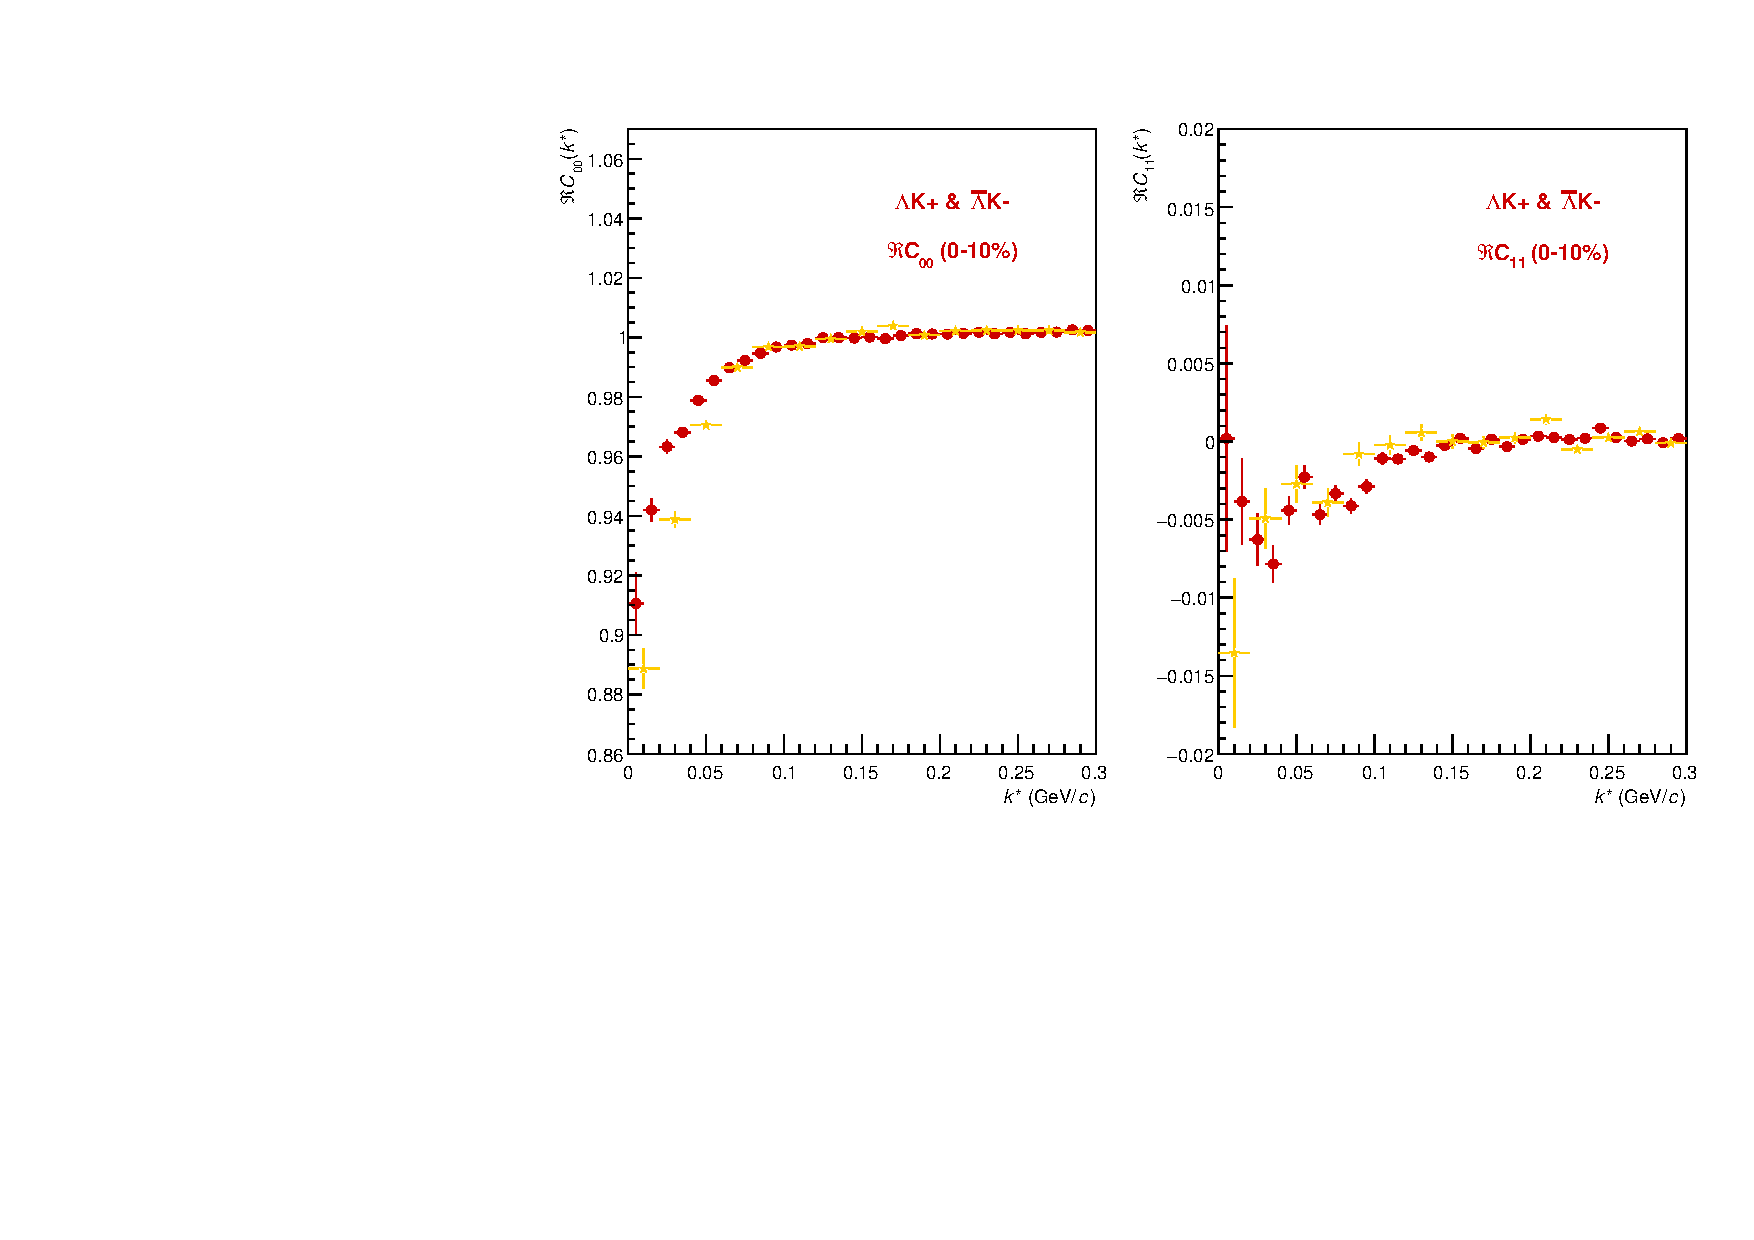
\includegraphics[width=\textwidth]{\ResultsDirBase Results_cLamcKch_20181205/SphericalHarmonics/LamKchP/CanCfYlmReC00C11_LamKchPALamKchM_0010.pdf}
  \caption[\LamKchP $C_{00}$ and $\Im C_{11}$ Spherical Harmonic Components (0-10\%)]{$C_{00}$ (left) and $\Im C_{11}$ (right) components of a spherical harmonic decomposition of the \LamKchP correlation function for the 0-10\% centrality bin.  
The $C_{00}$ component is similar to the 1D correlation functions typically studied, and probes the overall size of the source.
The $\Im C_{11}$ component probes the asymmetry in the system; a non-zero value reveals the asymmetry}
  \label{fig:LamKchP_ReC00C11_0010}
\end{figure}


Fig. \ref{fig:LamKchP_StdThermSources} shows a closer look at the THERMINATOR simulation, whose spherical harmonic decomposition was shown along with the data in Fig. \ref{fig:LamKchP_ReC00C11_0010}.
The top left of Fig. \ref{fig:LamKchP_StdThermSources_Spatial} shows a fit to the one-dimensional correlation function from THERMINATOR.
The scattering parameters are known precisely here, as they served as the weights used in the simulation, and are kept constant in the fit.
We are interested in looking at the extracted one-dimensional source size here, so the $\lambda$ parameter is also fixed at unity.
The other three plots in Fig. \ref{fig:LamKchP_StdThermSources_Spatial} show the source distribution in the out (top right), side (bottom left), and long (bottom right) directions (all in the PRF).
The source distributions have all been fitted with a Gaussian form, the result of which is printed within the respective plot.
One immediately sees a significant shift in the out direction, $\mu_{\mathrm{out}} \approx$ 4 fm, and negligible shift in the other two directions, $\mu_{\mathrm{side}} \approx \mu_{\mathrm{long}} \approx$ 0 fm.
The figure demonstrates that, within the THERMINATOR model, the \Lam is, on average, emitted further out that its K partner.
Finally, Fig. \ref{fig:LamKchP_StdThermSources_Temporal} shows the distribution of the relative time of emittance, again in the PRF.
The figure shows that the \Lam is, on average, emitted earlier than its K partner.



\begin{figure}[h!]
  \centering
  %%----start of first subfigure---  
  \subfloat[Caption 1]{
    \label{fig:LamKchP_StdThermSources_Spatial}
    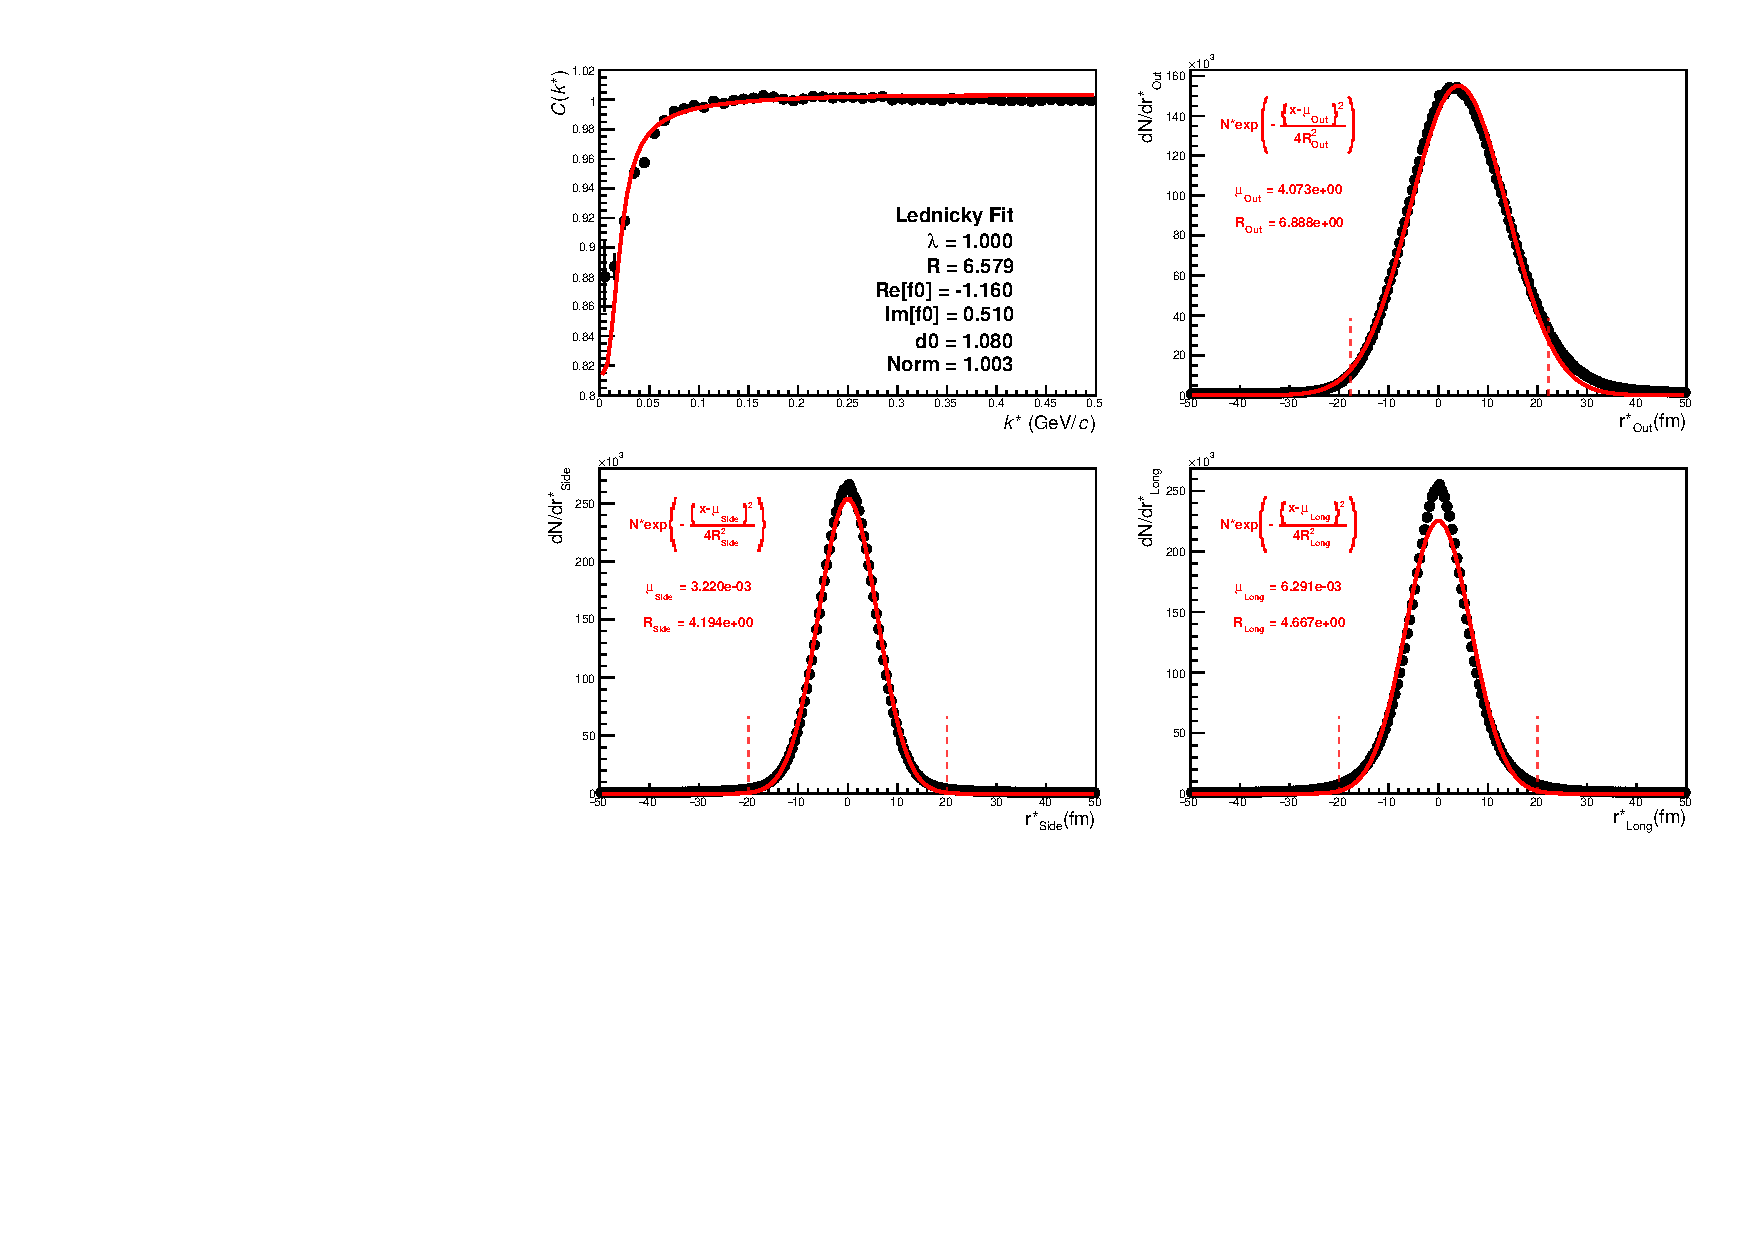
\includegraphics[width=\linewidth]{/home/jesse/Analysis/FemtoAnalysis/AnalysisNotes/7_ResultsAndDiscussion/7.1_ResultsLamK/7.1.5_ResultsLamK_DiscussionOfmTScaling/ThermPlots/LamKchP/CanCfwSource_Full_LamKchP_3dHistPairSource3d_oslLamKchP_FromFileCorrelationFunctions_wOtherPairs.pdf}} \\
  %%----start of second subfigure---
  \subfloat[Caption 2]{
    \label{fig:LamKchP_StdThermSources_Temporal}
    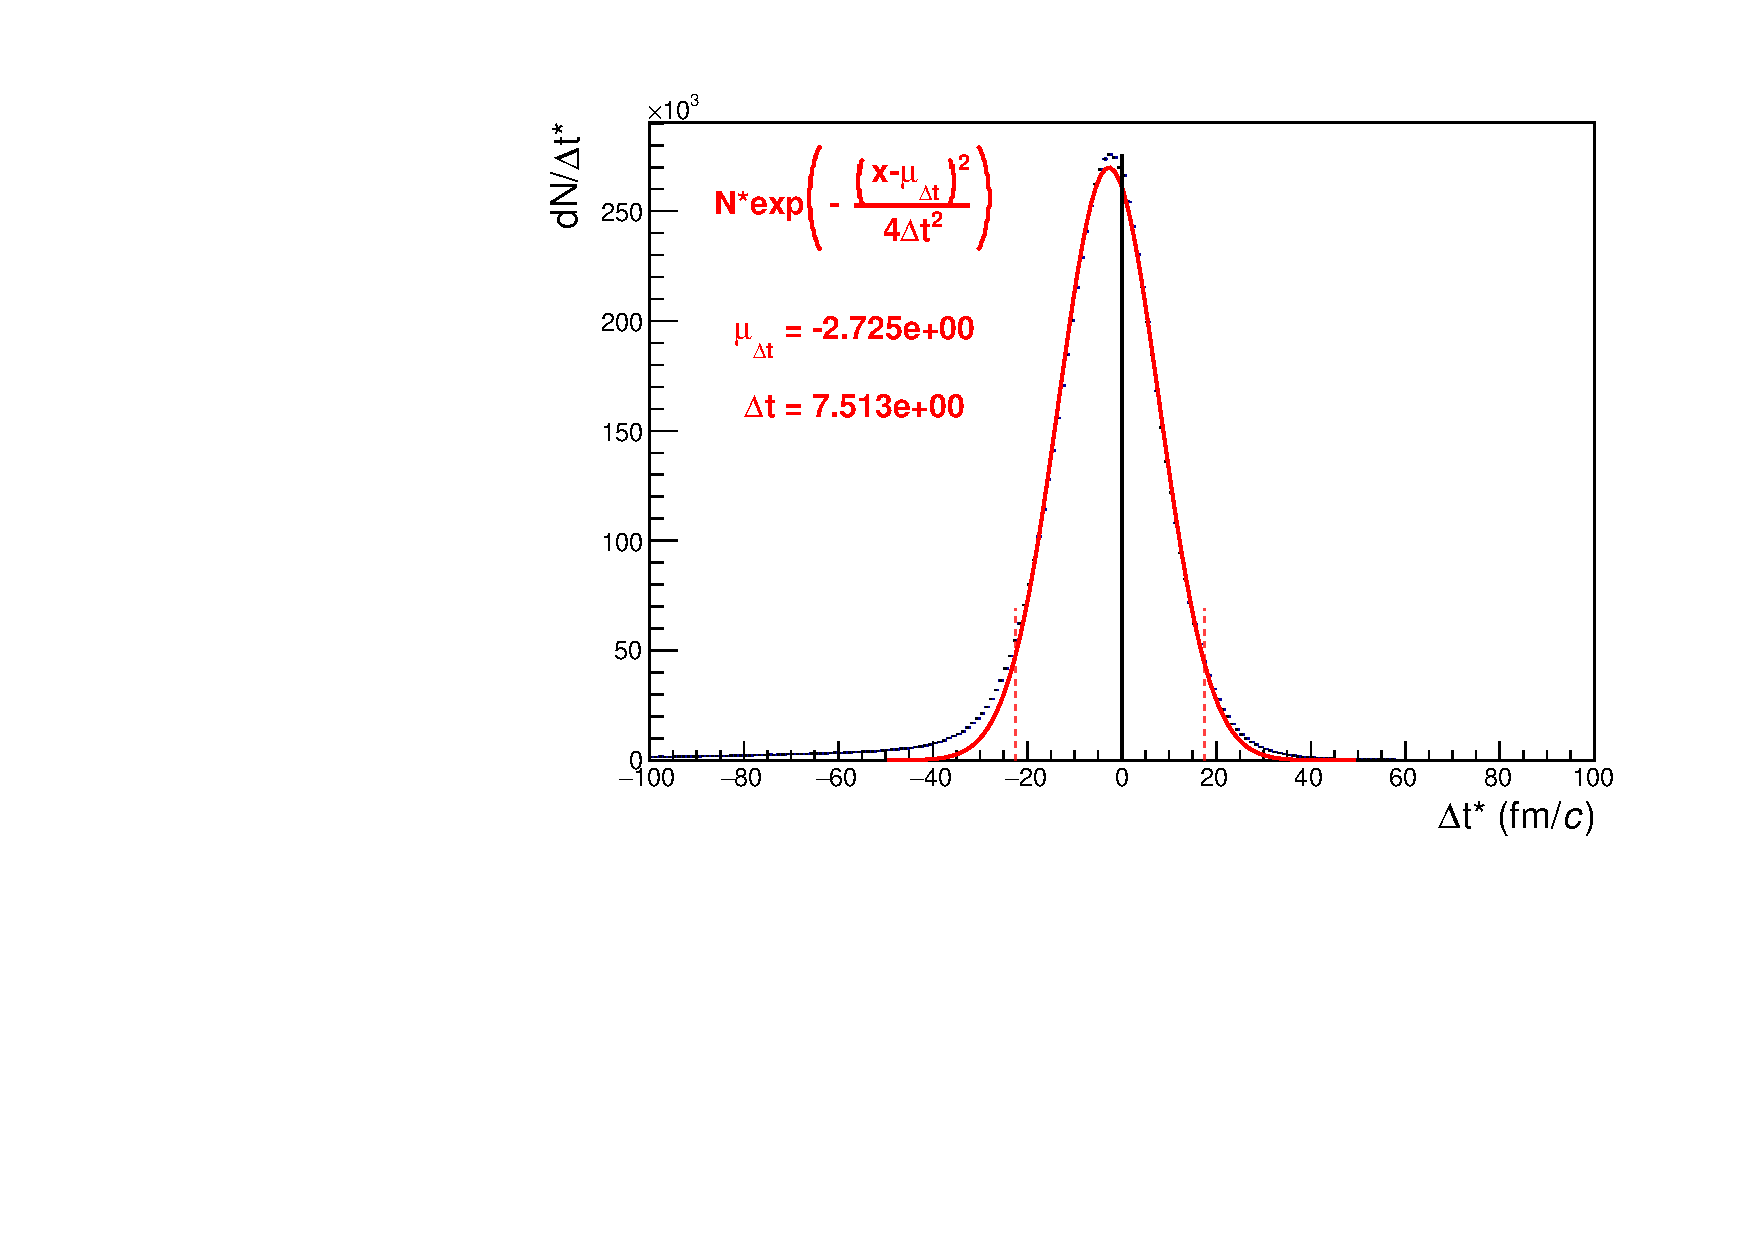
\includegraphics[width=0.60\linewidth]{/home/jesse/Analysis/FemtoAnalysis/AnalysisNotes/7_ResultsAndDiscussion/7.1_ResultsLamK/7.1.5_ResultsLamK_DiscussionOfmTScaling/ThermPlots/LamKchP/CanDeltaT_Full_LamKchP_FromFileCorrelationFunctions_wOtherPairs_BuildCfYlm.pdf}}  
  %%----overall caption----
  \caption[Short Overall]{Long Overall}
  \label{fig:LamKchP_StdThermSources}
\end{figure}




We end this section with a brief look at how a spatial separation of the single particle sources affects the radii extracted from a femtoscopic analysis.
To achieve this, we use THERMINATOR in a similar fashion as described above, but with one important difference.
Instead of taking the source information from THERMINATOR, we instead draw the source from a pre-determined Gaussian distribution.
In all cases, we take $R_{\mathrm{out}} = R_{\mathrm{side}} = R_{\mathrm{long}}$ = 5 fm, and $\mu_{\mathrm{side}} = \mu_{\mathrm{long}}$ = 0 fm.
Figure \ref{fig:LamKchP_ThermSources_GaussianSourceEx} shows an example of results obtained from THERMINATOR following this procedure, where $\mu_{\mathrm{out}}$ = 3 fm.









\begin{figure}[h]
  \centering
  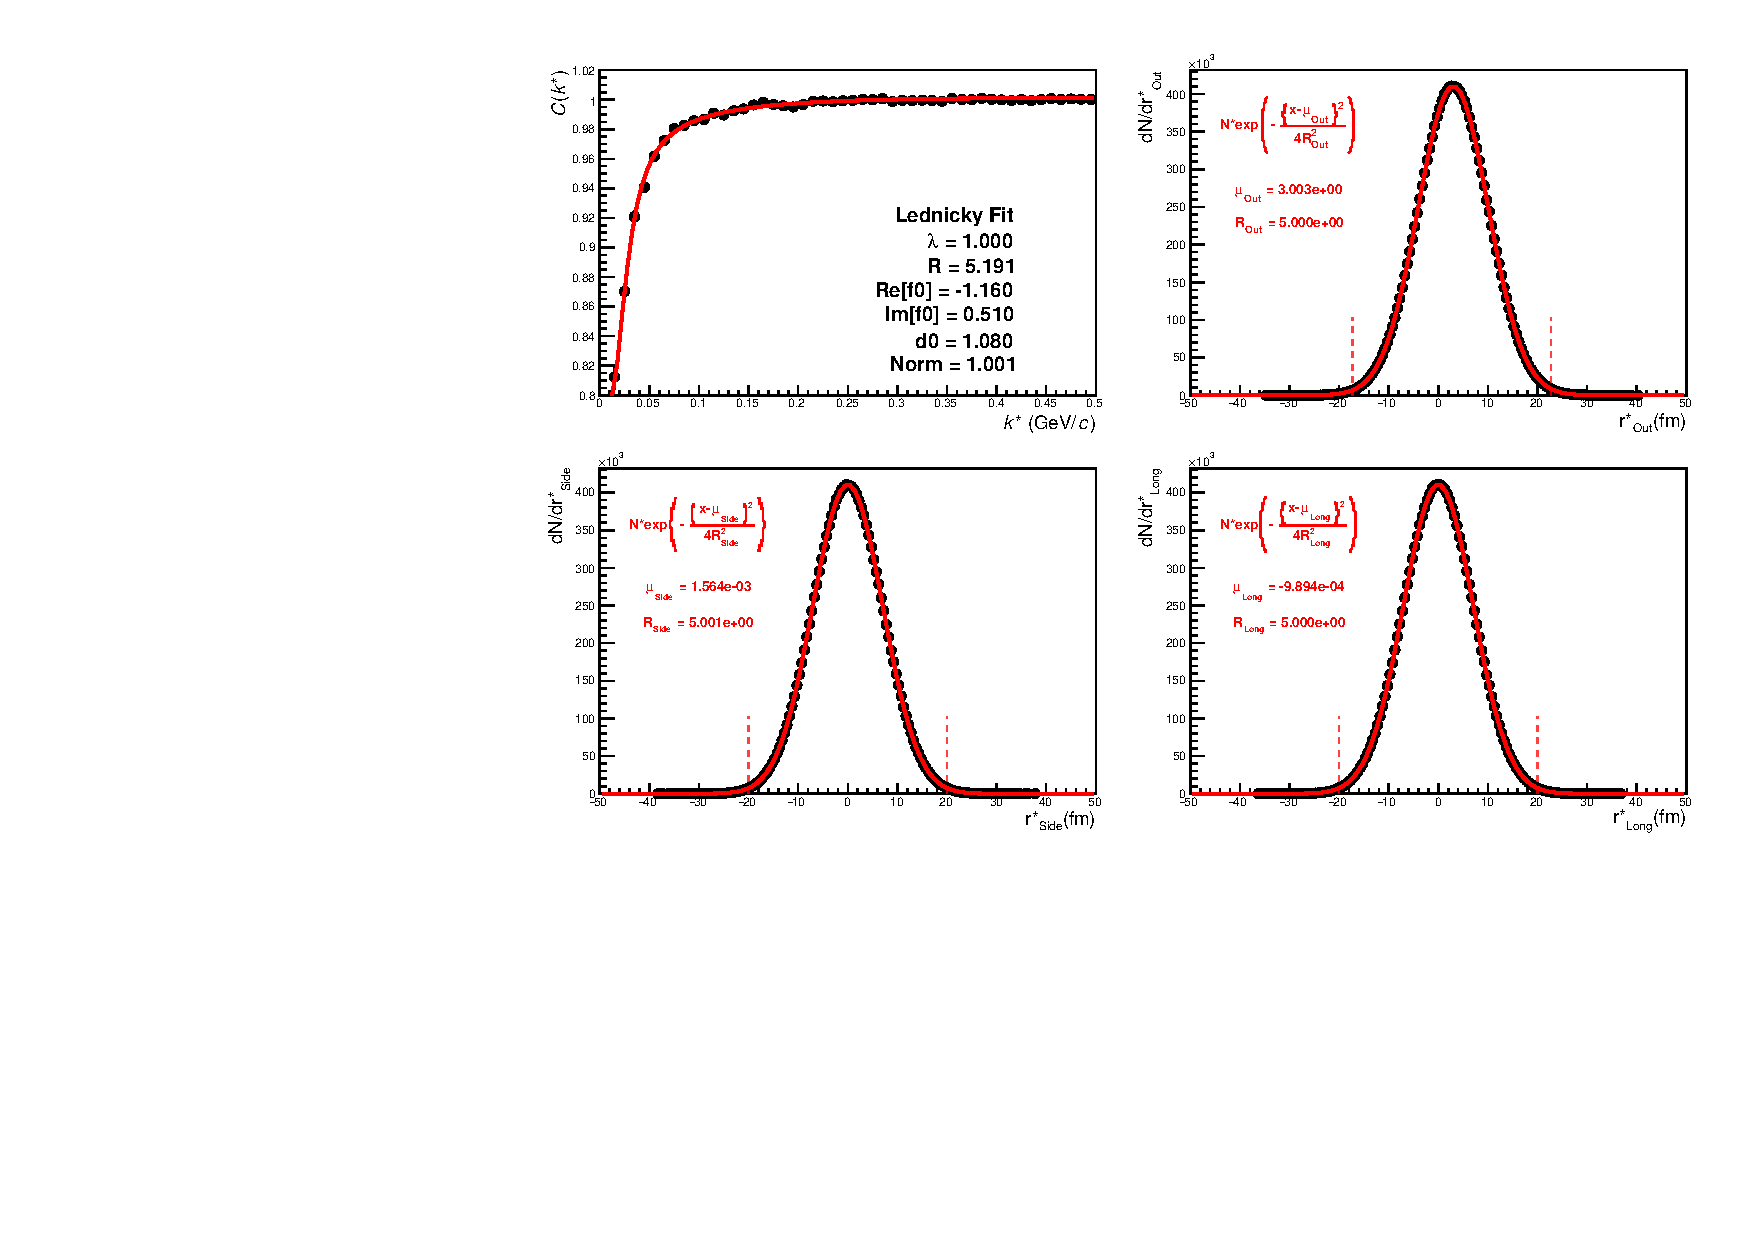
\includegraphics[width=\textwidth]{/home/jesse/Analysis/FemtoAnalysis/AnalysisNotes/7_ResultsAndDiscussion/7.1_ResultsLamK/7.1.5_ResultsLamK_DiscussionOfmTScaling/ThermPlots/LamKchP/CanCfwSource_Full_LamKchP_3dHistPairSource3d_oslLamKchP_FromFileCorrelationFunctions_wOtherPairs_DrawRStarFromGaussian_BuildCfYlm_cLamcKchMuOut3_cLamK0MuOut3_KchPKchPR538.pdf}
  \caption[Short Caption]{Long Caption}
  \label{fig:LamKchP_ThermSources_GaussianSourceEx}
\end{figure}


In Figure \ref{fig:LamKchP_ThermSources_VaryMuOut}, we show results for the case of $\mu_{out}$ = 1 fm, $\mu_{out}$ = 3 fm, and $\mu_{out}$ = 6 fm.
In this figure, we do not show the side and long distributions, as they appear identical to those shown in Fig. \ref{fig:LamKchP_ThermSources_GaussianSourceEx}.
The figure demonstrates that as the separation $\mu_{out}$ increases, so do the extracted femtoscopic radii.



\begin{figure}[h]
  \centering
  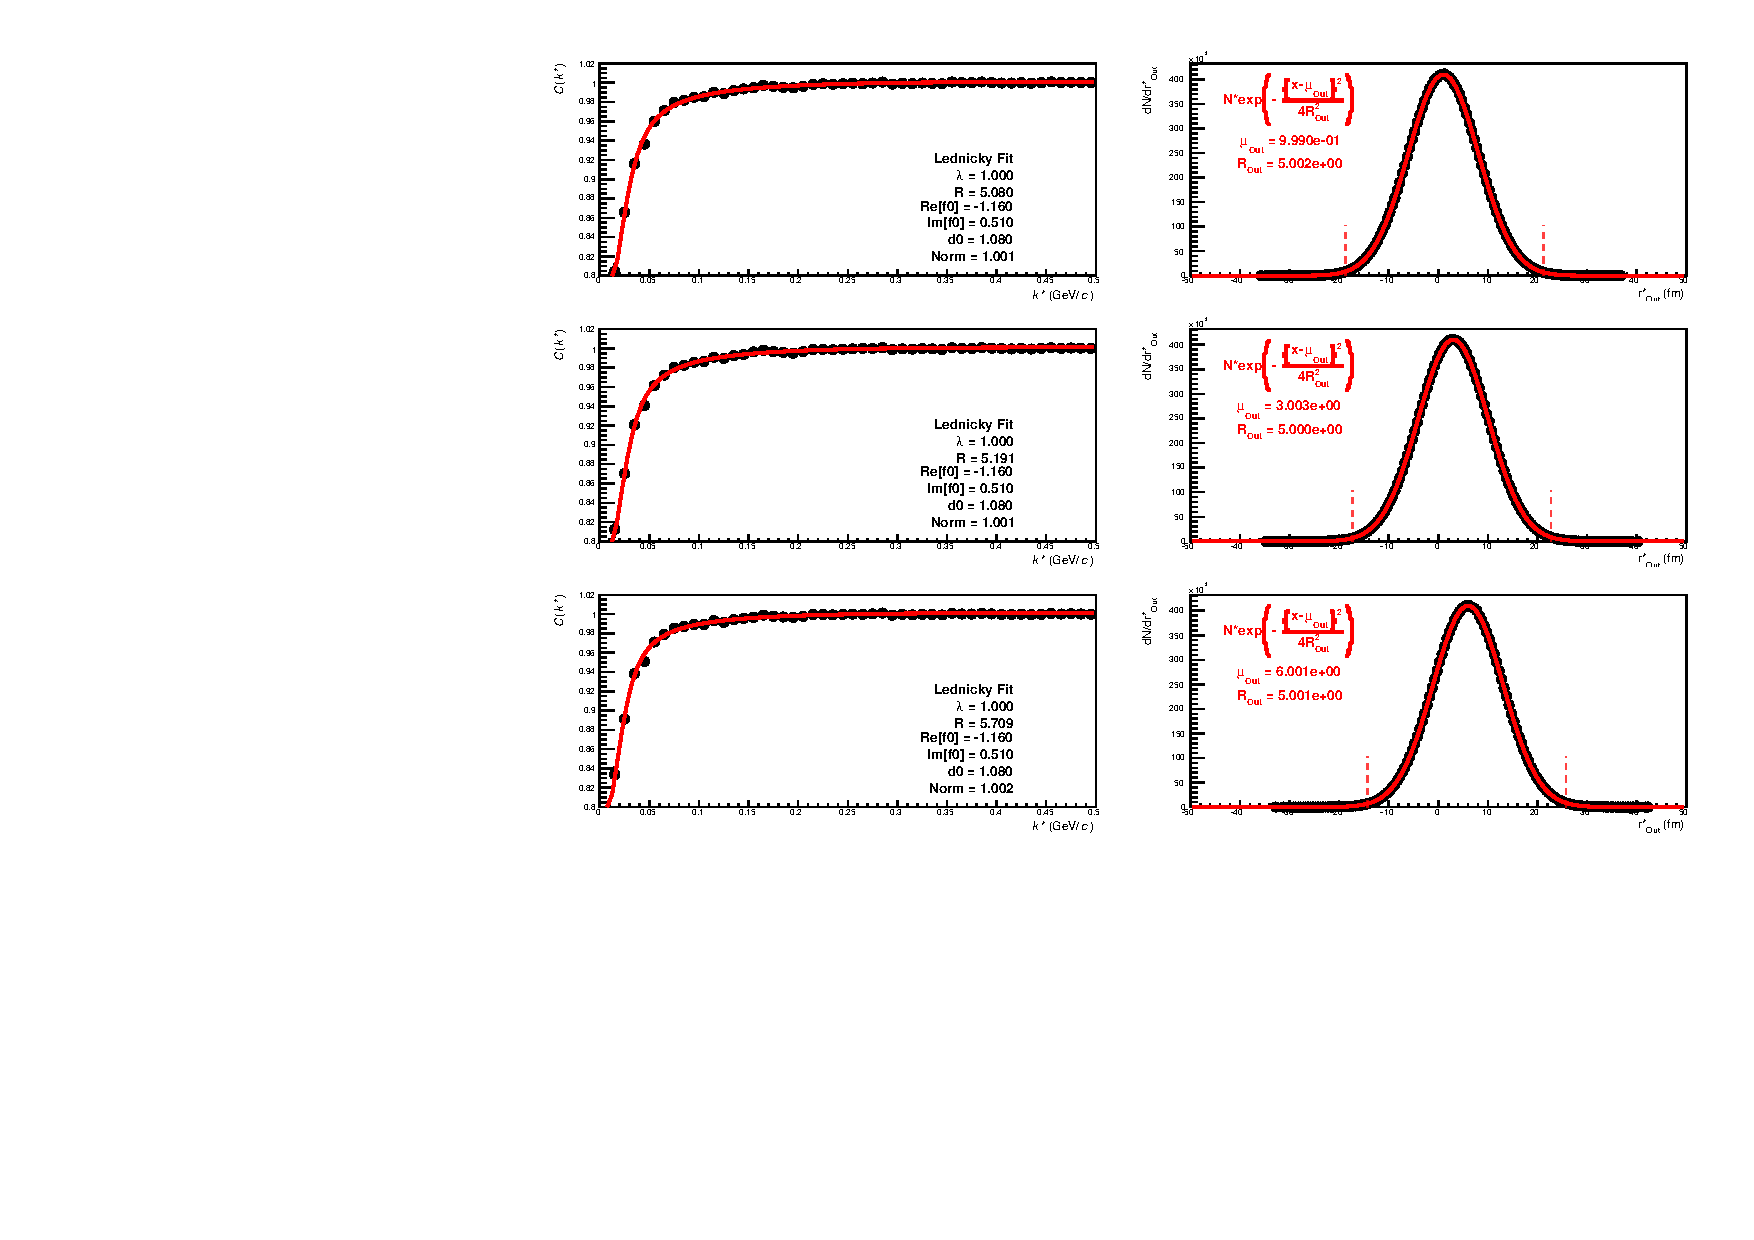
\includegraphics[width=\textwidth]{/home/jesse/Analysis/FemtoAnalysis/AnalysisNotes/7_ResultsAndDiscussion/7.1_ResultsLamK/7.1.5_ResultsLamK_DiscussionOfmTScaling/ThermPlots/LamKchP/CanCompMus_Full_LamKchP_3dHistPairSource3d_oslLamKchP.pdf}
  \caption[Short Caption]{Long Caption}
  \label{fig:LamKchP_ThermSources_VaryMuOut}
\end{figure}

















\clearpage
\end{document}